\hypertarget{(chap:capitolo6)}{}
\chapter{Risultati sperimentali}
In questo capitolo andremo a vedere i risultati sperimentali per ogni metodo.
\section{Risultati preprocessing matrici grezze}
Nelle sezione successive andremo a vedere i risultati delle valutazioni di ciascun modello rispetto la metrica $AUC$ e la $NDCG$ con $k\in \{5, 10, 25, 100\}$, in particolare la metrica che riteniamo sia più significativa è la seconda in quanto si basa sul ranking degli item nella lista $TopN$. \\
Per i confronti abbiamo scelto di usare $NDCG$ con $k=25$. Nei seguenti grafici

\subsection{Risultati base}
In questa sezione andremo a vedere i risultati del modello MostPop e del VAECF, che verranno utilizzati come bound per valutare quelli succcessivi. 

\subsubsection{MostPop}
Come detto il modello MostPop restituisce per ogni user la stessa lista di item più popolari.
Andiamo a vedere i risultati per dataset sul validation set:\\

\begin{tabular}{|l|c|cccc|}
    \toprule
    $dataset$ &    $AUC$ &  $NDCG@10$ & $NDCG@100$  & $NDCG@25$ & $NDCG@5$  \\
    \midrule
    macchine & 0.7644 & 0.1263 &   0.2414 &  0.1647 & 0.0920 \\
    ricambi  & 0.3427 &  0.0299 &   0.0732 &  0.0358 & 0.0000 \\
    totale  & 0.2810 &  0.0733 &   0.0811 &  0.0627 & 0.0360 \\

\bottomrule
\end{tabular}\\

Useremo questi risultati come bound per quelli degli altri modelli (MF, UserKnn), nel caso in cui questi siano migliori si procederà al tuning dei parametri e al calcolo finale dei risultati sul test set.\\
Quelli riportati qui di seguito sono i risultati del MostPop sul test set.\\

\begin{tabular}{|l|c|cccc|}
    \toprule
    $dataset$ &    $AUC$ &  $NDCG@10$ & $NDCG@100$  & $NDCG@25$ & $NDCG@5$  \\
    \midrule
    macchine & 0.7897 &  0.1364 &   0.2610 &  0.1875 & 0.1001 \\
    ricambi  & 0.3924 &  0.0753 &   0.1365 &  0.0793 & 0.0619 \\
    totale  & 0.3101 &  0.0807 &   0.1281 &  0.0866 & 0.0944 \\

\bottomrule
\end{tabular}

\subsubsection{VAECF}
Il modello VAECF è un modello che funziona su rating impliciti, la fase preliminare ha richiesto il tuning dei parametri riportati di seguito:
\begin{itemize}
    \item $n_{int}$ è la dimensione della rappresentazione latente interna, i possibili valori sono $\{5,10,15,20,50\}$;
    \item $n_{hid}$ è il numero di neuroni del layer dell'encoder e del decoder, i valori possibili sono $\{10,20,30,50,100,200\}$;
    \item $f_{act}$ è la funzione di attivazione applicata nei layer nascosti, che può essere una delle seguenti $\{sigmoid, tanh, elu, relu, relu6\}$.
\end{itemize}
\begin{minipage}[H]{0.45\textwidth}
    \begin{tabular}{|l|ccc|}
        \toprule
        $dataset$ &    $n_{int}$ &  $n_{hid}$ & $act\_f$ \\
        \midrule
        macchine & 5 & 30 & relu \\
        ricambi  &	5 & 30 & sigmoid\\
        totale  & 5 & 30 & sigmoid\\
    \bottomrule
    \end{tabular}\\
\end{minipage}
\begin{minipage}[H]{0.55\textwidth}
    Il tuning dei parametri ha portato a considerare tutte le possibili combinazioni dei parametri sopra citati, andiamo a vedere per ogni dataset quali parametri hanno restituito sul validation set i risultati migliori.
\end{minipage}\\

Andiamo a vedere i risultati per dataset sul validation set dopo il tuning dei parametri:\\

\begin{tabular}{|l|c|cccc|}
    \toprule
    $dataset$ &    $AUC$ &  $NDCG@10$ & $NDCG@100$  & $NDCG@25$ & $NDCG@5$  \\
    \midrule
    macchine & 0.8201 & 0.1768 & 0.3032 & 0.2282 & 0.1325 \\
    ricambi & 0.4773 & 0.0452 & 0.1052 & 0.0643 & 0.0506 \\
    totale  & 0.4190 & 0.0980 & 0.0941 & 0.0741 & 0.1208 \\
\bottomrule
\end{tabular}\\

Dato che i risultati della tabella precedente sono quelli del validation set su un modello con parametri ottimizzati, non possiamo direttamente usarli per il confronto con 

Vediamo i risultati del modello validato sul test set:\\

\begin{tabular}{|l|c|cccc|}
    \toprule
    $dataset$ &    $AUC$ &  $NDCG@10$ & $NDCG@100$  & $NDCG@25$ & $NDCG@5$  \\
    \midrule
    macchine & 0.8269 &  0.1948 &   0.3301 &  0.2487 & 0.1473 \\
    ricambi  & 0.4930 &  0.0919 &   0.1401 &  0.1075 & 0.0801 \\
    totale  & 0.4343 &  0.0874 &   0.1398 &  0.0964 & 0.0988 \\

\bottomrule
\end{tabular}

\subsection{Risultati MF e UserKnn}
In questa sezione andremo a vedere per ogni tecnica di preprocessing adottata sulle matrici grezze i risultati ottenuti.
La valutazione si è divisa in due fasi: 
\begin{enumerate}
    \item preliminare: confrontiamo i risultati dei modelli (MF, UserKnn) con parametri di default sulle matrici dei rating, con il risultato bound dato dal MostPop;
    \item avanzata: dopo aver effettuato il tuning sui parametri dei modelli con le matrici rimanenti, si confrontano con il bound dato dal VAECF. 
\end{enumerate} 
Cominceremo prima con la tecnica basata su min-max, poi con quella ordered-based per concludere infine con quella basata sui prodotti totali. 
Spesso si farà riferimenti ai risultati dei modelli, intendendo il risultato dato dei modelli basato sulle diverse matrici dei rating.

\subsubsection{Normalizzazione min-max}
Come spiegato nel capitolo dedicato alle tecniche ora andremo ad osservare i risultati rispetto diversi gruppi di triplette.

\paragraph{Gruppo globale}
In questa sezione vedremo la normalizzazione min-max applicata al gruppo user-based, ossia quello dove ciascun gruppo contiene solo le triplette di un singolo user.
Nella tabella sottostante possiamo vedere sulle righe i dataset (macchine, ricambi, totale), mentre sulle righe possiamo vedere le \textit{espressioni d'intresse}. Ciascun grafico poi mostra sulle ascisse la $scale$ della matrice dei rating e sulle ordinate il risultato ottenuto da tale matrice rispetto la metrica $NDCG@25$. La linea tratteggiata blu rappresenta il risultato del modello MostPop che viene usato come bound.
Inoltre i puntini di colore blu rappresentano i risultati forniti dal modello MF, mentre quelli arancioni dallo UserKnn.

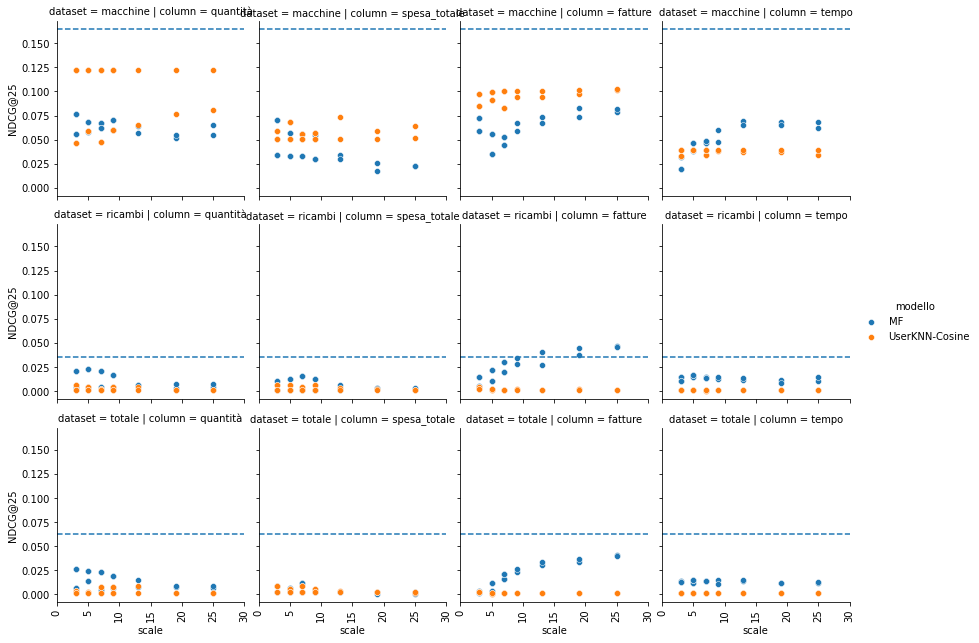
\includegraphics[width=16cm]{figures/risultati_minmax_globale.png}

Possiamo vedere come quasi tutti i grafici riportino risultati scarsi, questo ci fa pensare che questo approcio almeno al gruppo globale non sia funzionale allo scopo.
L'unico grafico che riporta qualche risultato sopra il bound è quello nell'incrocio (ricambi-numero fatture), potrebbe essere che il numero di fatture sia un modo migliore di descrivere gli acquisti degli item rispetto per esempio la quantità o la soesa totale.
Vediamo i risultati dopo il tuning dei parametri.

\paragraph{Gruppi user-based}
In questa sezione vedremo la normalizzazione min-max applicata al gruppo user-based, ossia quello dove ciascun gruppo contiene solo le triplette di un singolo user.
Nella tabella sottostante possiamo vedere sulle righe i dataset (macchine, ricambi, totale), mentre sulle righe possiamo vedere le \textit{espressioni d'intresse}. Ciascun grafico poi mostra sulle ascisse la $scale$ della matrice dei rating e sulle ordinate il risultato ottenuto da tale matrice rispetto la metrica $NDCG@25$. La linea tratteggiata blu rappresenta il risultato del modello MostPop che viene usato come bound.
Inoltre i puntini di colore blu rappresentano i risultati forniti dal modello MF, mentre quelli arancioni dallo UserKnn.

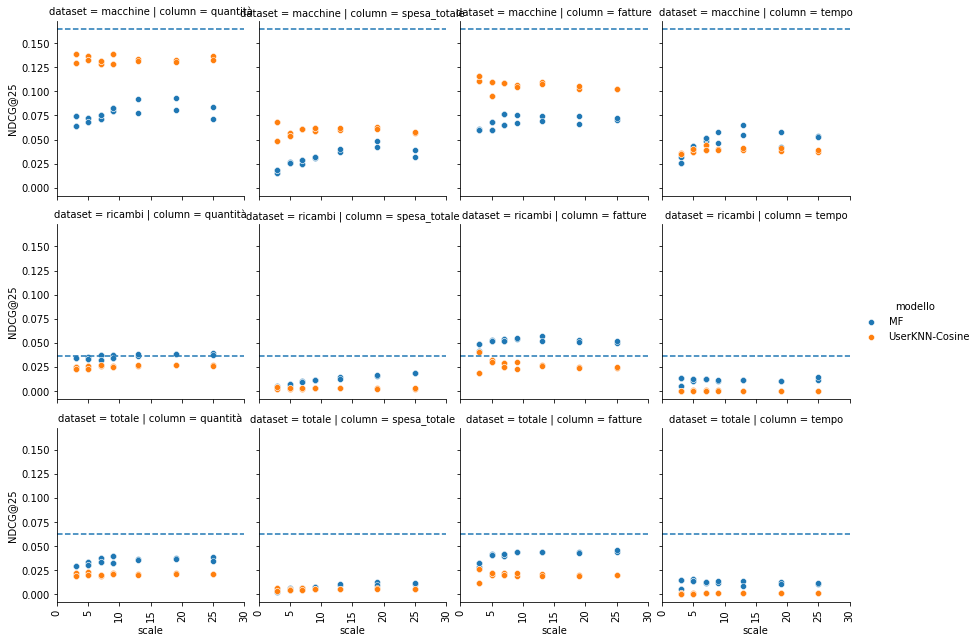
\includegraphics[width=16cm]{figures/risultati_minmax_singolo.png}

Come possiamo vedere come quasi tutti i risultati sono al di sotto del bound a parte che nell'incrocio: dataset ricambi - espressione d'interesse numero di fatture, probabilmente vale quanto detto per il caso precedente.
\begin{minipage}[H]{0.45\textwidth}
    
\end{minipage}
\begin{minipage}[H]{0.45\textwidth}
    
\end{minipage}
\paragraph{Gruppo user-category-based}
\begin{comment}
Nel seguente caso vedremo invece la tecnica applicata solo al dataset totale, possiamo vedere che ci sono sei colonne, le prime tre dividono gli item rispetto le categoria dei tre livelli della gerarchia prodotto, mentre i secondi tre dividono le macchine rispetto la la gerarchia prodotto e i ricambi rispetto il gruppo merceologico.\\ 
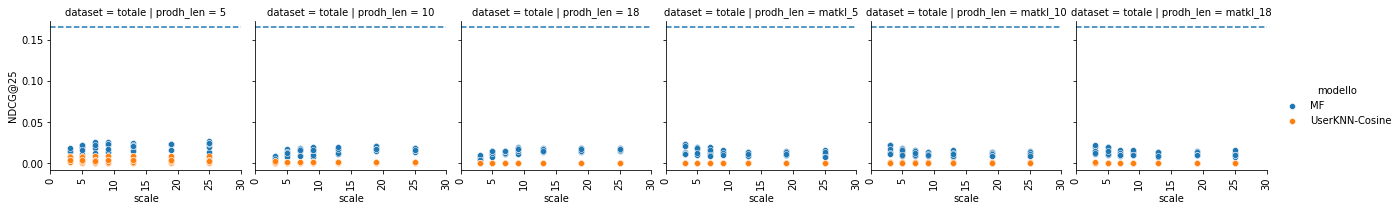
\includegraphics[width=16cm]{figures/risultati_minmax_categoria.png}

Possiamo vedere come confrontare i prodotti rispetto 
\end{comment}

\subsubsection{Tecnica ordered-based}

\paragraph{Gruppo globale}
In questa sezione vedremo la tacnica di preprocessing ordered-based applicata al gruppo globale, ossia quello contenente tutte le triplette.
Nella tabella sottostante possiamo vedere sulle righe i dataset (macchine, ricambi, totale), mentre sulle righe possiamo vedere le \textit{espressioni d'intresse}. Ciascun grafico poi mostra sulle ascisse la $scale$ della matrice dei rating e sulle ordinate il risultato ottenuto da tale matrice rispetto la metrica $NDCG@25$. La linea tratteggiata blu rappresenta il risultato del modello MostPop che viene usato come bound.
Inoltre i puntini di colore blu rappresentano i risultati forniti dal modello MF, mentre quelli arancioni dallo UserKnn.

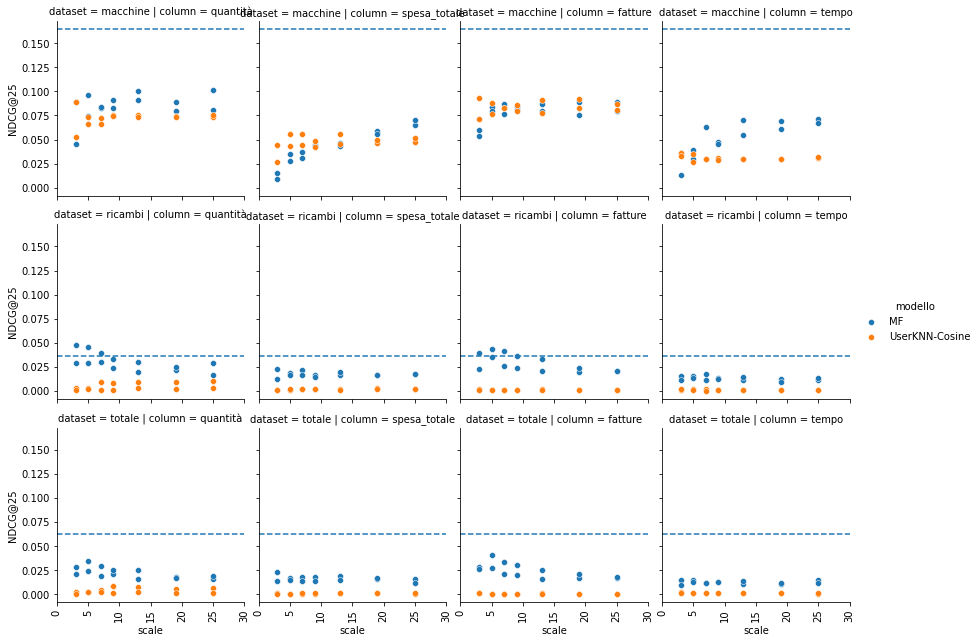
\includegraphics[width=16cm]{figures/risultati_ordered_globale.png}

Nella tabella di grafici sopra riportati possiamo vedere sulle righe i dataset (macchine, ricambi, totale), mentre sulle colonne possiamo vedere le espressioni d'interesse (quantità, )

\paragraph{Gruppi user-based}
Di seguito possiamo vedere i risultati relativi la tecnica ordered-based su gruppi di triplette appartenenti allo stesso user.\\
I grafici sono organizzati come segue: sulle righe i dataset (macchine, ricambi, totale), mentre sulle righe possiamo vedere le \textit{espressioni d'intresse}. Ciascun grafico poi mostra sulle ascisse la $scale$ della matrice dei rating e sulle ordinate il risultato ottenuto da tale matrice rispetto la metrica $NDCG@25$. La linea tratteggiata blu rappresenta il risultato del modello MostPop che viene usato come bound.
Inoltre i puntini di colore blu rappresentano i risultati forniti dal modello MF, mentre quelli arancioni dallo UserKnn.\\

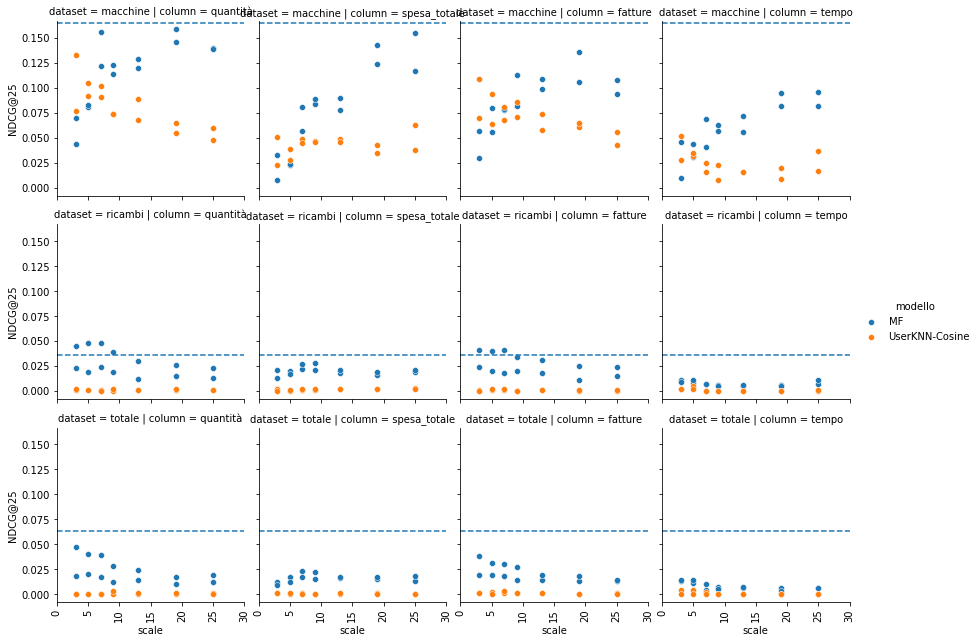
\includegraphics[width=16cm]{figures/risultati_ordered_singolo.png}

Possiamo vedere come il metodo non funzioni se non per alcuni risultati nell'incrocio (ricambi,quantità) che superano di poco il livello bound.

\paragraph{Gruppo user-category-based}
\begin{comment}
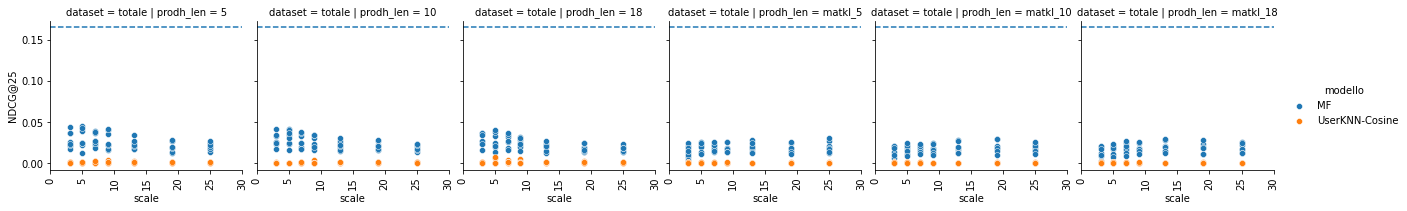
\includegraphics[width=16cm]{figures/risultati_ordered_categoria.png}
\end{comment}
\subsubsection{Tecnica product-based}

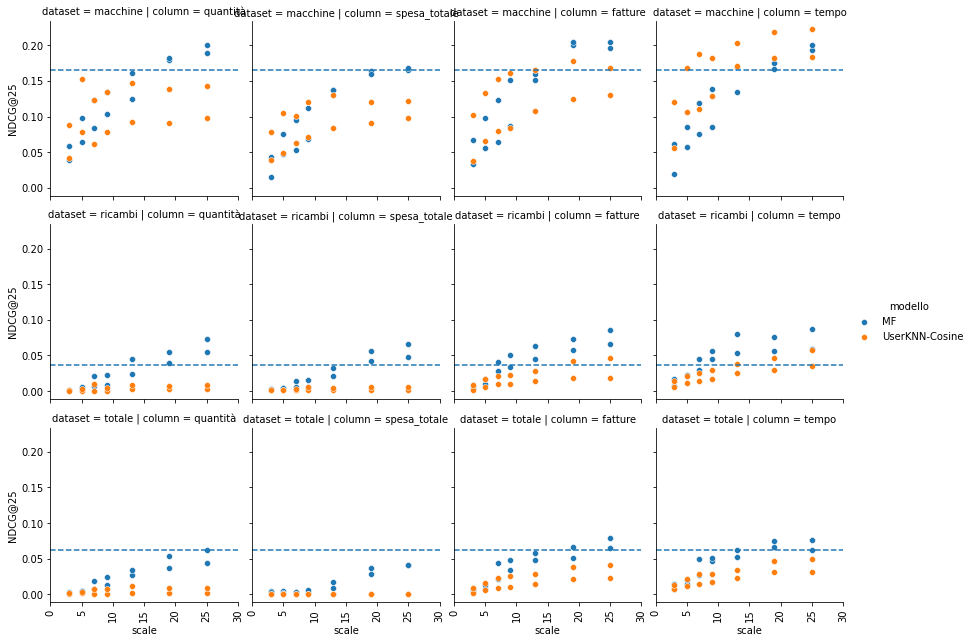
\includegraphics[width=16cm]{figures/prodotto.png}

\section{Risultati matrici grezze combinate}
Vediamo di seguito i risultati delle versioni combinate.

\subsection{Combinazione liste \textit{TopN}}
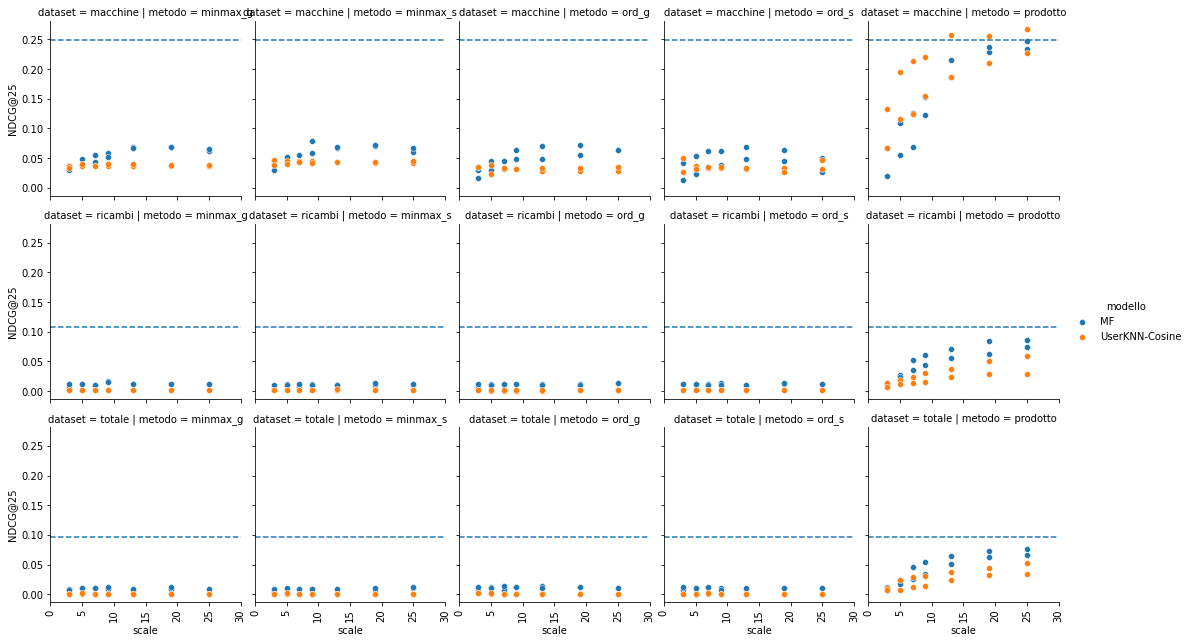
\includegraphics[width=16cm]{figures/comb_1.png}

\subsection{Media matrici dei rating}
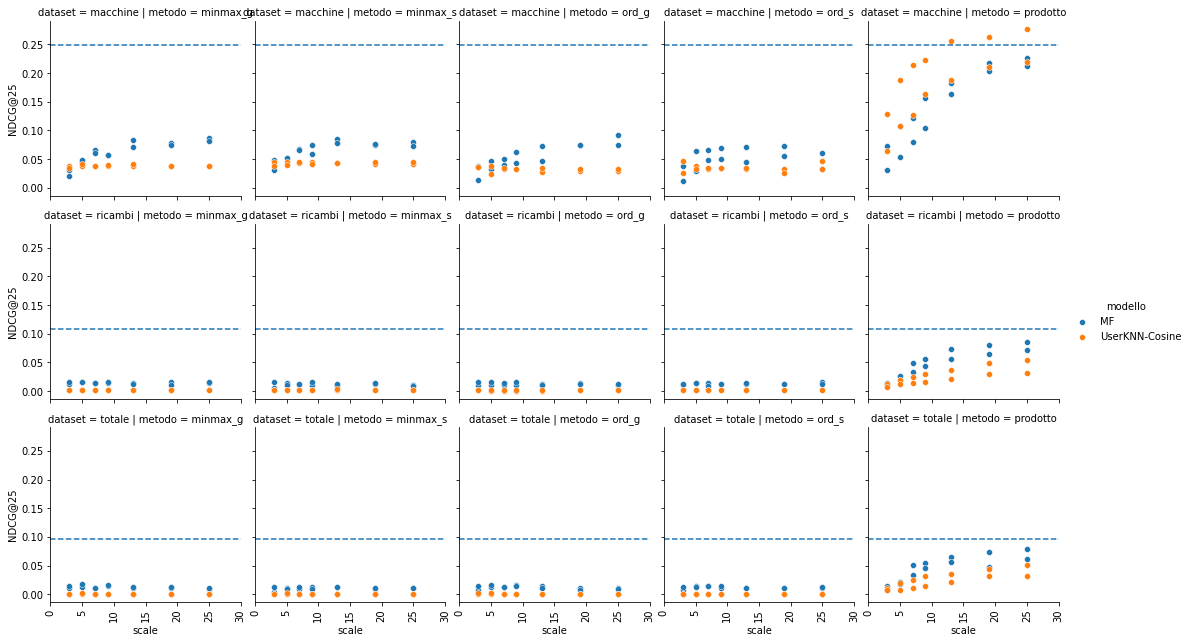
\includegraphics[width=16cm]{figures/comb_2.png}

\section{Esperimenti con approccio next-basket}
In questa sezione vedremo i risultati dell'approccio next-based. Per prima cosa andiamo a vedere quali sono stati i parametri selezionati con il tuning per ciascun dataset.\\

\begin{minipage}[H]{0.45\textwidth}
    \begin{tabular}{|l|ccc|}
        \toprule
        $dataset$ &    $\alpha$ &  $q$ & $r$ \\
        \midrule
        macchine & 0.5 & 100 & $\infty$ \\
        ricambi  &	0.75 & 50 & $\infty$ \\
        totale  & 0 & 100 & $\infty$ \\
    \bottomrule
    \end{tabular}
\end{minipage}
\begin{minipage}[H]{0.55\textwidth}
    Possiamo vedere che alla fine il tuning ha portato ad avere una finestra di recentezza  $r = \infty$, quindi stiamo usando la popolarità \textit{popularity user-wise}. 
\end{minipage}\\

Possiamo inoltre vedere che la località $q$ è comunque alta, mentre per quanto riguarda $alpha$ abbiamo che le macchine calcolano la probabilità composta al 50\%, nei ricambi si da più importanza a quella dello user in esame, ed infine nel totale si considera solo la probabilità composta dello user esterno.

Vediamo i risultati sperimentali con i modelli ottimizzati sul validation set:\\

\begin{tabular}{|l|cccc|}
    \toprule
    $dataset$  &  $NDCG@5$ & $NDCG@10$  & $NDCG@25$ & $NDCG@100$  \\
    \midrule
    macchine & 0.5832 & 0.6278 & 0.6506 & 0.6627 \\
    ricambi & 0.1728 & 0.1892 & 0.2381 & 0.3317 \\
    totale  & 0.2196 & 0.2295 & 0.2834 & 0.3653 \\
\bottomrule
\end{tabular}\\

E ora i corrispondenti risultati con il test set:\\

\begin{tabular}{|l|cccc|}
    \toprule
    $dataset$  &  $NDCG@5$ & $NDCG@10$  & $NDCG@25$ & $NDCG@100$  \\
    \midrule
    macchine & 0.6049 & 0.6476 & 0.6726 & 0.6741 \\
    ricambi & 0.2261 & 0.2403 & 0.2915 & 0.3811 \\
    totale  & 0.1955 & 0.2045 & 0.2595 & 0.3537 \\
\bottomrule
\end{tabular}\\

Ricordiamo che questi risultati non sono confrontabili con quelli delle sezioni precendenti, però i risultati sembrano molti interessanti.